\documentclass[10pt,pdf,hyperref={unicode}]{beamer}

\mode<presentation>
{
\usetheme{boxes}
\beamertemplatenavigationsymbolsempty

\setbeamertemplate{footline}[page number]
\setbeamersize{text margin left=0.5em, text margin right=0.5em}
}

\usepackage[utf8]{inputenc}
\usepackage[english, russian]{babel}
\usepackage{bm}
\usepackage{multirow}
\usepackage{ragged2e}
\usepackage{indentfirst}
\usepackage{multicol}
\usepackage{subfig}
\usepackage{amsmath,amssymb}
\usepackage{enumerate}
\usepackage{mathtools}
\usepackage{comment}
\usepackage{multicol}
\usepackage[all]{xy}

\newcommand{\bz}{\mathbf{z}}
\newcommand{\bx}{\mathbf{x}}
\newcommand{\by}{\mathbf{y}}
\newcommand{\bv}{\mathbf{v}}
\newcommand{\bw}{\mathbf{w}}
\newcommand{\ba}{\mathbf{a}}
\newcommand{\bb}{\mathbf{b}}
\newcommand{\bff}{\mathbf{f}}
\newcommand{\bh}{\mathbf{h}}
\newcommand{\bl}{\mathbf{l}}
\newcommand{\bp}{\mathbf{p}}
\newcommand{\bq}{\mathbf{q}}
\newcommand{\bs}{\mathbf{s}}
\newcommand{\bt}{\mathbf{t}}
\newcommand{\bu}{\mathbf{u}}
\newcommand{\bT}{\mathbf{T}}
\newcommand{\bX}{\mathbf{X}}
\newcommand{\bZ}{\mathbf{Z}}
\newcommand{\bS}{\mathbf{S}}
\newcommand{\bH}{\mathbf{H}}
\newcommand{\bW}{\mathbf{W}}
\newcommand{\bY}{\mathbf{Y}}
\newcommand{\bU}{\mathbf{U}}
\newcommand{\bQ}{\mathbf{Q}}
\newcommand{\bP}{\mathbf{P}}
\newcommand{\bA}{\mathbf{A}}
\newcommand{\bB}{\mathbf{B}}
\newcommand{\bC}{\mathbf{C}}
\newcommand{\bE}{\mathbf{E}}
\newcommand{\bF}{\mathbf{F}}
\newcommand{\bsigma}{\boldsymbol{\sigma}}
\newcommand{\bomega}{\boldsymbol{\omega}}
\newcommand{\btheta}{\boldsymbol{\theta}}
\newcommand{\bgamma}{\boldsymbol{\gamma}}
\newcommand{\bdelta}{\boldsymbol{\delta}}
\newcommand{\bPsi}{\boldsymbol{\Psi}}
\newcommand{\bpsi}{\boldsymbol{\psi}}
\newcommand{\bxi}{\boldsymbol{\xi}}
\newcommand{\bmu}{\boldsymbol{\mu}}
\newcommand{\bchi}{\boldsymbol{\chi}}
\newcommand{\bzeta}{\boldsymbol{\zeta}}
\newcommand{\blambda}{\boldsymbol{\lambda}}
\newcommand{\beps}{\boldsymbol{\varepsilon}}
\newcommand{\bZeta}{\boldsymbol{Z}}
% mathcal
\newcommand{\cX}{\mathcal{X}}
\newcommand{\cY}{\mathcal{Y}}
\newcommand{\cW}{\mathcal{W}}

\newcommand{\dH}{\mathds{H}}
\newcommand{\dR}{\mathds{R}}
% transpose
\newcommand{\T}{^{\mathsf{T}}}

\renewcommand{\epsilon}{\ensuremath{\varepsilon}}
\renewcommand{\phi}{\ensuremath{\varphi}}
\renewcommand{\kappa}{\ensuremath{\varkappa}}
\renewcommand{\le}{\ensuremath{\leqslant}}
\renewcommand{\leq}{\ensuremath{\leqslant}}
\renewcommand{\ge}{\ensuremath{\geqslant}}
\renewcommand{\geq}{\ensuremath{\geqslant}}
\renewcommand{\emptyset}{\varnothing}

\usepackage{tikz}
\usetikzlibrary{positioning,arrows}

\tikzstyle{name} = [parameters]
\definecolor{name}{rgb}{0.5,0.5,0.5}

\usepackage{caption}
\captionsetup{skip=0pt,belowskip=0pt}

\newtheorem{rustheorem}{Теорема}
\newtheorem{russtatement}{Утверждение}
\newtheorem{rusdefinition}{Определение}

% colors
\definecolor{darkgreen}{rgb}{0.0, 0.2, 0.13}
\definecolor{darkcyan}{rgb}{0.0, 0.55, 0.55}

\AtBeginEnvironment{figure}{\setcounter{subfigure}{0}}

\captionsetup[subfloat]{labelformat=empty}
\addto\captionsrussian{\renewcommand{\figurename}{}}
\graphicspath{{../figures/}}

%----------------------------------------------------------------------------------------------------------

\title[Заголовок]{Способы учёта шума данных в модели \\ нейронных дифференциальных уравнений}
\author{Владимиров Э.А.}

\institute[]{Московский физико-технический институт}
\date[2022]{\small \today}

%---------------------------------------------------------------------------------------------------------
\begin{document}

\begin{frame}
\titlepage
\end{frame}

%----------------------------------------------------------------------------------------------------------
\begin{frame}{Удаление шума}
	\begin{alertblock}{Проблема}
		Удаления шума из временного ряда для стабилизации модели предсказания.
	\end{alertblock}
	
	\begin{alertblock}{Задача}
		Внедрить методы фильтрации временных рядов в фреймворк Neural ODE
	\end{alertblock}
	
	\begin{alertblock}{Решение}
		Использование фреймворка Neural SDE.
	\end{alertblock}
\end{frame}

%---------------------------------------------------------------------------------------------------------
\begin{frame}{Методы фильтрации и Neural ODE}
	\begin{figure}
		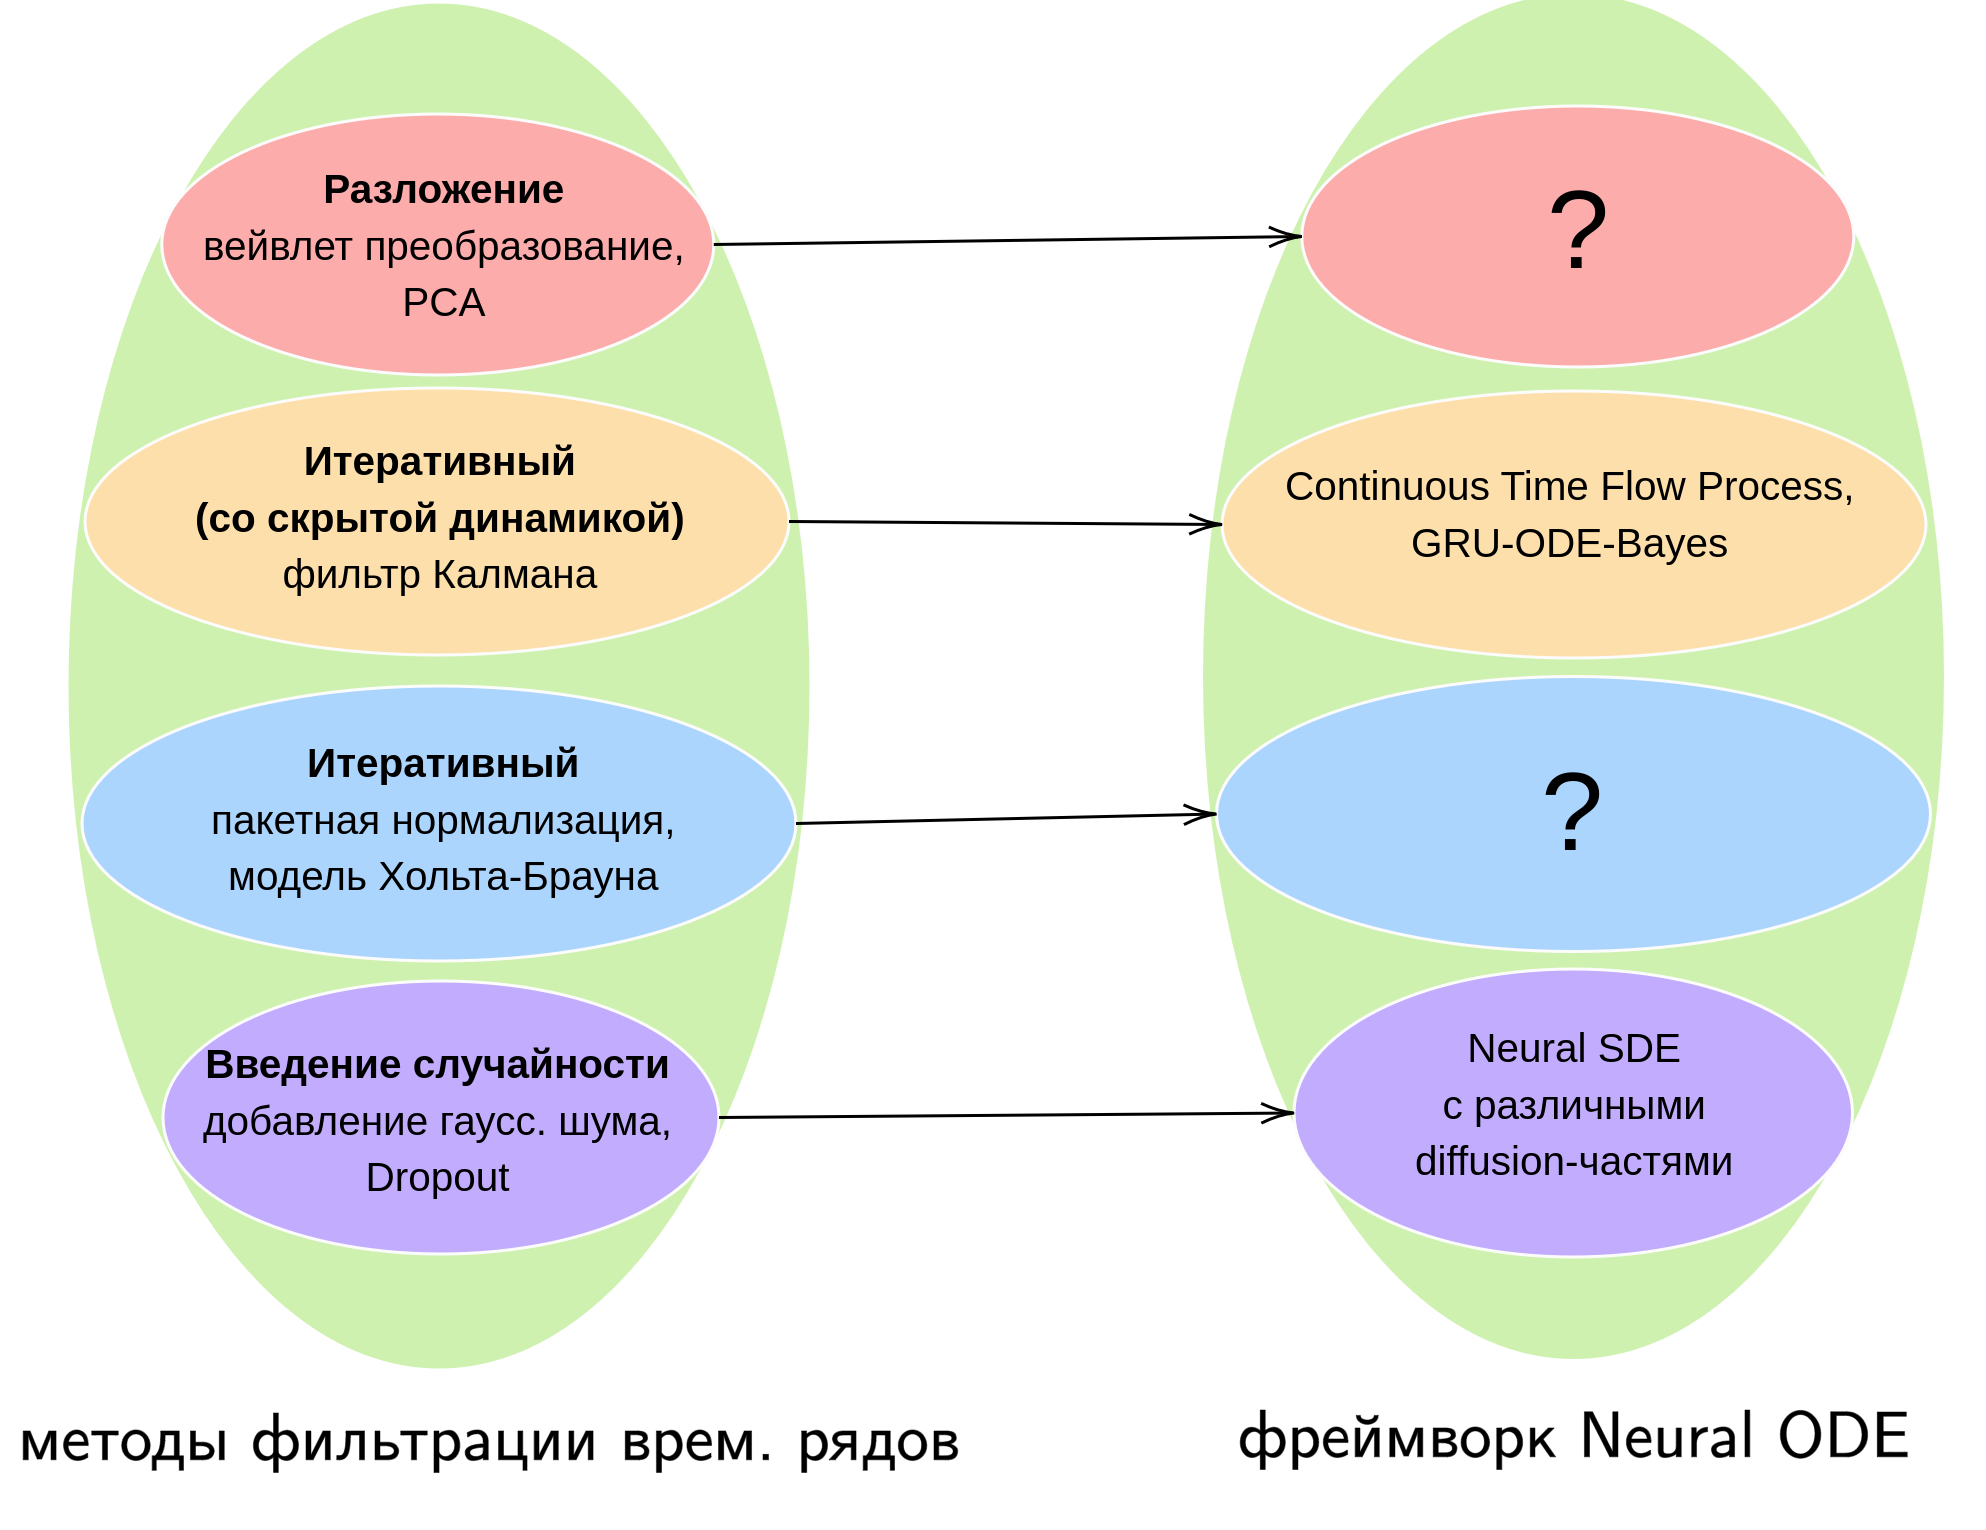
\includegraphics[width=0.85\textwidth]{3rd_slide.png}
	\end{figure}
\end{frame}

%---------------------------------------------------------------------------------------------------------
\begin{frame}{Neural ODE and Neural SDE}
	Модель Neural ODE аппроксимирует отображение $\bx \rightarrow \by$ путём обучения нейронной сети $f_\theta$ и линейных отображений $l_\theta^1, \, l_\theta^2$.
	$$ \by \approx l_\theta^2(\bh_T), \text{ где } \bh_T = \bh_0 + \int_{0}^{T} f_\theta(\bh_t) dt \text{ и } \bh_0 = l_\theta^1(\bx)$$
	
	Модель Neural SDE имеет следующий вид:
	$$ \bh_0 = \zeta_\theta(V), \quad d\bh_t = \mu_\theta(t, \bh_t)dt + \sigma_\theta(t, \bh_t) \circ d\bW_t, \quad \widehat{\bY_t} = l_\theta(\bh_t),$$
	где $\zeta_\theta, \mu_\theta, \sigma_\theta$ ~--- нейронные сети, $l_\theta$ ~--- линейное преобразование, $(\bW_t, t \in [0, T])$  ~--- винеровский процесс и $V \sim \mathcal{N}(0, I_v)$ ~--- стандартный гауссовский вектор.
	
	Решением SDE служит случайный процесс $(\bh_t, t \in [0, T])$.
	\bigskip
	\footnotetext[1]{\textit{David Duvenaud, Ricky T. Q. Chen, Yulia Rubanova, Jesse Bettencourt} Ordinary Differential Equations. UNITEXT - La Matematica per il 3 piu 2, 109(NeurIPS):31–60, 2018.}
	\footnotetext[2]{\textit{Xuanqing Liu, Tesi Xiao, Si Si, Qin Cao, Sanjiv Kumar, and Cho-Jui Hsieh.} Neural SDE: Stabilizing Neural ODE Networks with Stochastic Noise. (2), 2019.}
\end{frame}

%----------------------------------------------------------------------------------------------------------
\begin{frame}{Вычислительный эксперимент}
	\begin{alertblock}{Цель}
		 Показать, что качество модели Neural ODE уменьшается при наличии шума в данных.
	\end{alertblock}
	
	\begin{multicols}{2}
		\begin{figure}
			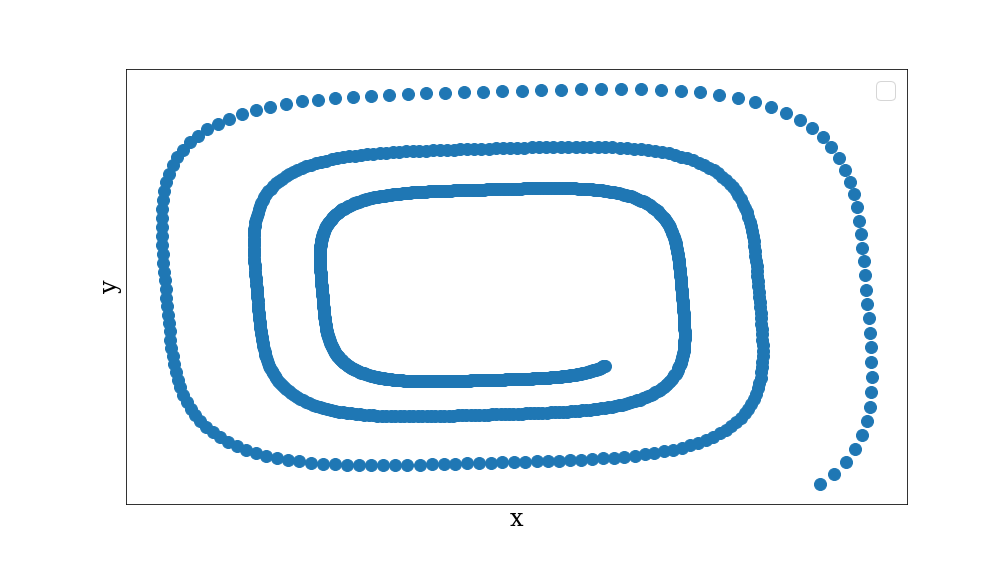
\includegraphics[width=0.5\textwidth]{Spirals.png}
			\caption{Временной ряд "Спираль"}
		\end{figure}
		
		\begin{figure}[bhtp]
			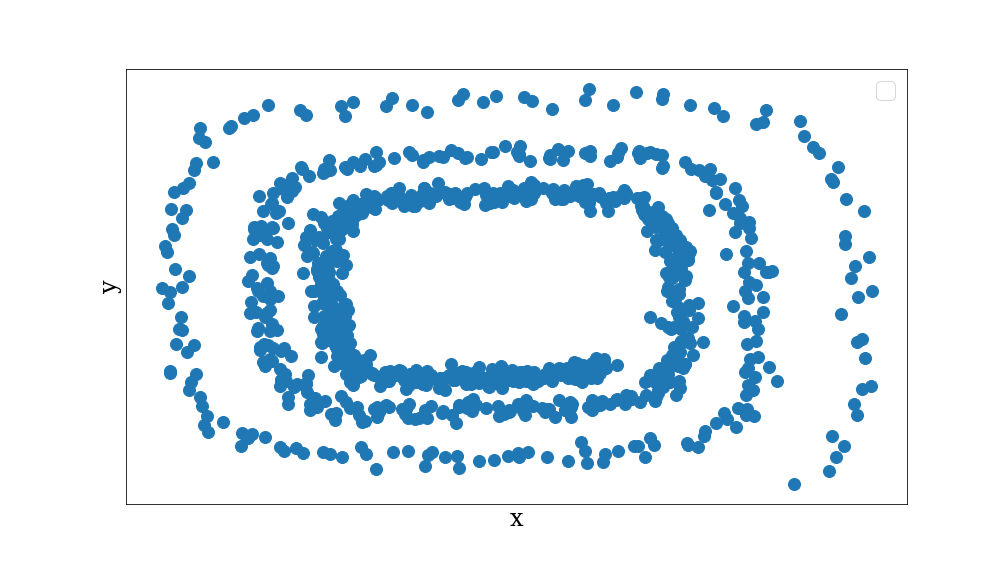
\includegraphics[width=0.5\textwidth]{Noisy spirals.png}
			\caption{Зашумлённая спираль}
		\end{figure}
	\end{multicols}
	
\end{frame}

%----------------------------------------------------------------------------------------------------------
\begin{frame}{Анализ ошибки}
	\begin{multicols}{2}
		\begin{figure}
			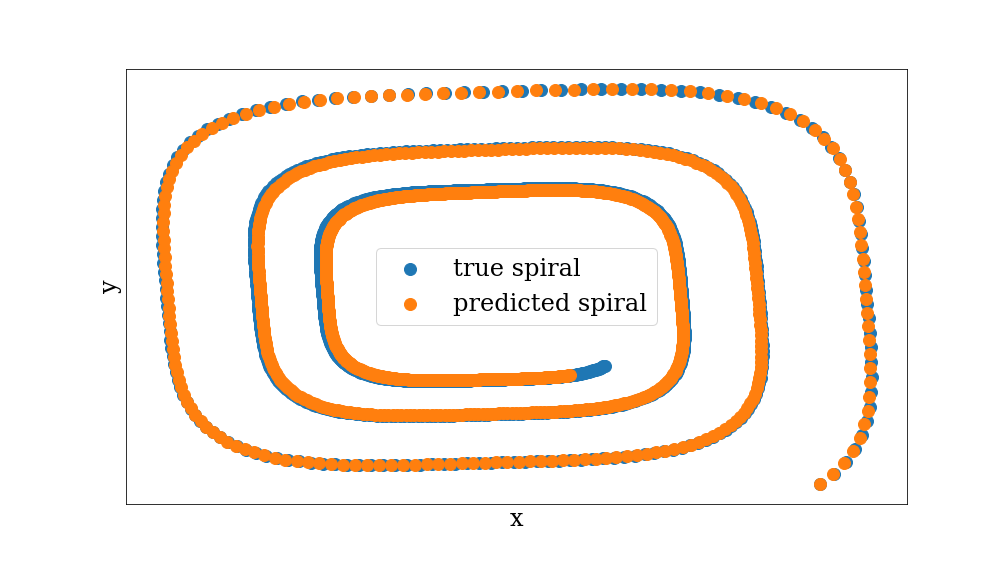
\includegraphics[width=0.5\textwidth]{Spirals vs ODE Spirals.png}
			\caption{NODE на чистых данных}
		\end{figure}
		
		\begin{figure}[bhtp]
			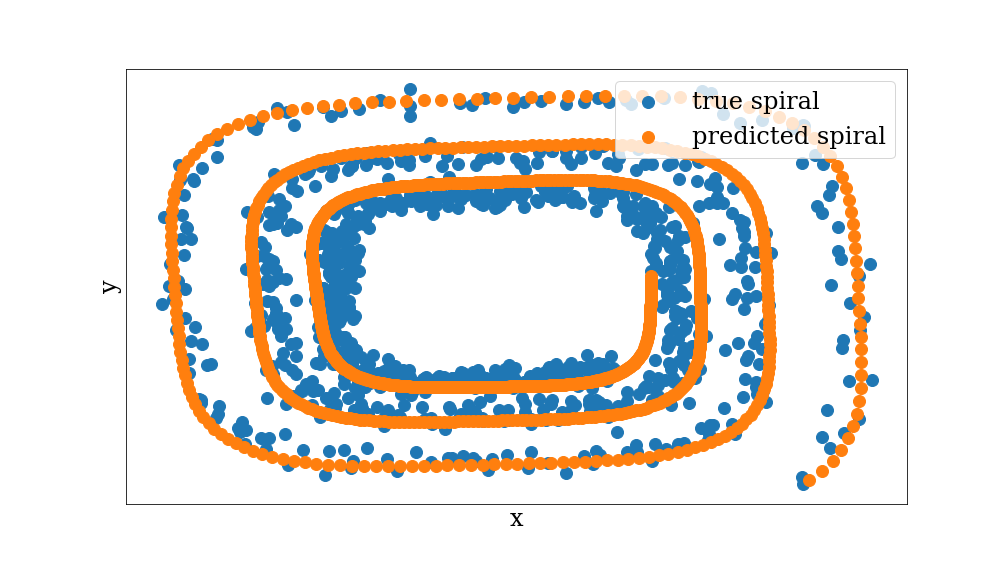
\includegraphics[width=0.5\textwidth]{Noisy Spirals vs ODE Spirals.png}
			\caption{NODE на зашумлённых данных}
		\end{figure}
	\end{multicols}
\end{frame}

\begin{frame}{Анализ ошибки}
	\begin{figure}[bhtp]
		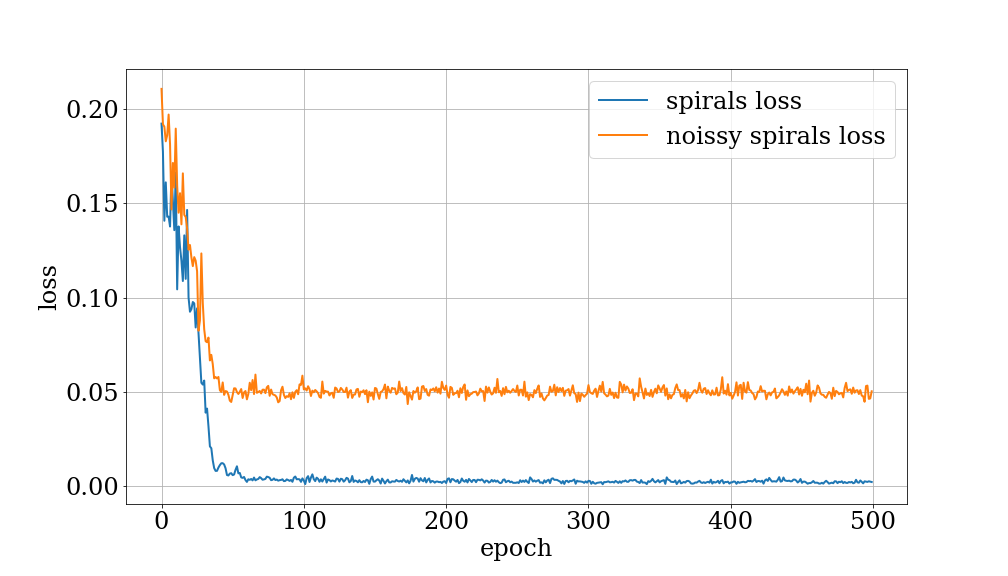
\includegraphics[width=0.95\linewidth]{train_losses.png}
		\caption{Функция потерь при обучении Neural ODE \\ на незашумлённых и зашумлённых данных}
	\end{figure}
\end{frame}

%----------------------------------------------------------------------------------------------------------
\begin{frame}{Заключение}
	\begin{enumerate}
		\item Предоставлена классификация методов фильтрации временных рядов
		
		\item Показано, что модель Neural ODE работает хуже на зашумлённых данных
		
	\end{enumerate}
\end{frame}
%----------------------------------------------------------------------------------------------------------

\end{document} 